\documentclass[10pt]{book}

%These tell TeX which packages to use.
\usepackage{array,epsfig}
\usepackage{amsmath}
\usepackage{amsfonts}
\usepackage{amssymb}
\usepackage{amsxtra}
\usepackage{amsthm}
\usepackage{mathrsfs}
\usepackage{color}
\usepackage{multicol}
\usepackage{enumitem}
%\usepackage{mdframed}
\usepackage[most]{tcolorbox}
\usepackage{pgfplots}
\usetikzlibrary{arrows}
\pgfplotsset{compat=1.6}

\pgfplotsset{soldot/.style={color=black,only marks,mark=*}} \pgfplotsset{holdot/.style={color=black,fill=white,only marks,mark=*}}

%Here I define some theorem styles and shortcut commands for symbols I use often
\theoremstyle{definition}
\newtheorem{defn}{Definition}
\newtheorem{thm}{Theorem}
\newtheorem{cor}{Corollary}
\newtheorem*{rmk}{Remark}
\newtheorem{lem}{Lemma}
\newtheorem*{joke}{Joke}
\newtheorem{ex}{Example}
\newtheorem*{soln}{Solution}
\newtheorem{prop}{Proposition}

\newcommand{\lra}{\longrightarrow}
\newcommand{\ra}{\rightarrow}
\newcommand{\surj}{\twoheadrightarrow}
\newcommand{\graph}{\mathrm{graph}}
\newcommand{\bb}[1]{\mathbb{#1}}
\newcommand{\Z}{\bb{Z}}
\newcommand{\Q}{\bb{Q}}
\newcommand{\R}{\bb{R}}
\newcommand{\C}{\bb{C}}
\newcommand{\N}{\bb{N}}
\newcommand{\M}{\mathbf{M}}
\newcommand{\m}{\mathbf{m}}
\newcommand{\MM}{\mathscr{M}}
\newcommand{\HH}{\mathscr{H}}
\newcommand{\Om}{\Omega}
\newcommand{\Ho}{\in\HH(\Om)}
\newcommand{\bd}{\partial}
\newcommand{\del}{\partial}
\newcommand{\bardel}{\overline\partial}
\newcommand{\textdf}[1]{\textbf{\textsf{#1}}\index{#1}}
\newcommand{\img}{\mathrm{img}}
\newcommand{\ip}[2]{\left\langle{#1},{#2}\right\rangle}
\newcommand{\inter}[1]{\mathrm{int}{#1}}
\newcommand{\exter}[1]{\mathrm{ext}{#1}}
\newcommand{\cl}[1]{\mathrm{cl}{#1}}
\newcommand{\ds}{\displaystyle}
\newcommand{\vol}{\mathrm{vol}}
\newcommand{\cnt}{\mathrm{ct}}
\newcommand{\osc}{\mathrm{osc}}
\newcommand{\LL}{\mathbf{L}}
\newcommand{\UU}{\mathbf{U}}
\newcommand{\support}{\mathrm{support}}
\newcommand{\AND}{\;\wedge\;}
\newcommand{\OR}{\;\vee\;}
\newcommand{\Oset}{\varnothing}
\newcommand{\st}{\ni}
\newcommand{\wh}{\widehat}
%Pagination stuff.
\setlength{\topmargin}{-0.75in}
\setlength{\oddsidemargin}{0in}
\setlength{\evensidemargin}{0in}
\setlength{\textheight}{9.in}
\setlength{\textwidth}{6.5in}
\pagestyle{empty}
\begin{document}
\begin{flushleft}
Name:\underline{\hspace{13cm}}Date:\underline{\hspace{2cm}}
\end{flushleft}
\begin{center}
{\Large Math 1041-012 \hspace{0.5cm} Section 4.9}
\end{center}
%\vspace{0.2 cm}

\begin{tcolorbox}
\subsection*{Definition}
A function $F$ is called an \underline{\hspace{5cm}} of $f$ on an interval $I$ if $F'(x)=f(x)$ for all $x$ in $I$.\\ \\
\textit{In other words:} Let $f$ be some function that is a \underline{derivative}:
\[
\frac{d}{dx}\left(\ ? \ \right)=f(x)
\]
the $?$ is the original function whose derivative is $f(x)$. 
\subsection*{Theorem}
If $F(x)$ is an antiderivative of $f(x)$ on an interval, then the most general antiderivative of $f(x)$ is
\[
F(x)+C,\textrm{ where $C$ is any constant.}
\]
\end{tcolorbox}
\begin{figure}[h!]
    \centering
    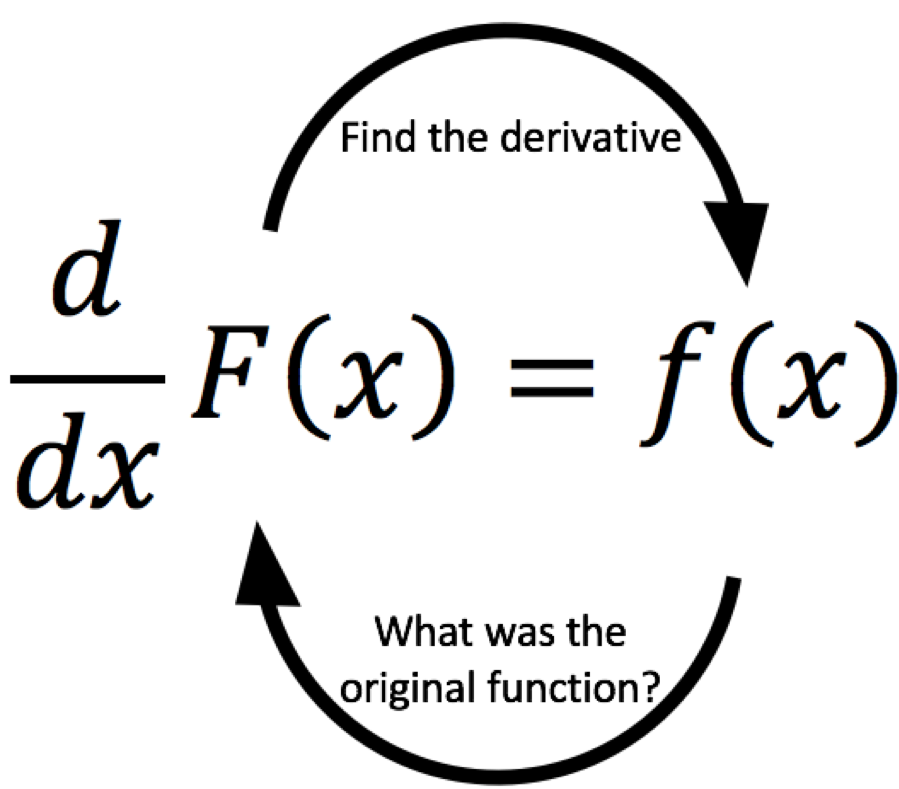
\includegraphics[width=6cm]{antiDer.png}
\end{figure}
\subsection*{Example 1: Short examples}
Find the most general antiderivative of each of the following functions.
 \begin{multicols}{2}
    \begin{enumerate}[label=(\alph*)]
        \item $f(x)=2x$\vspace{1cm}
        \item $f(x)=5$\vspace{1cm}
        \item $f(x)=\cos x$\vspace{1cm}
        \item $f(x)=-\sin x$\vspace{1cm}
        \item $\displaystyle f(x)=\frac{1}{x}$\vspace{1cm}
        \item $f(x)=e^x+2x$\vspace{1cm}
        \item $f(x)=\sec^2(x)$\vspace{1cm}
    \end{enumerate}
    \end{multicols}
\clearpage
\begin{figure}[ht]
    \centering
    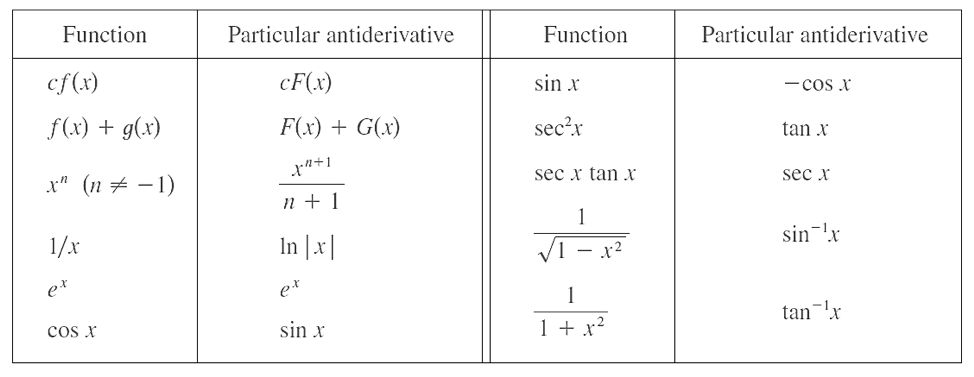
\includegraphics{Basic-AntiRules.png}
\end{figure}
\subsection*{Example 2}
Find all functions $g$ such that 
\[
g'(x)=4\sin x+\frac{2x^5-\sqrt{x}}{x}
\]
\vspace{5cm}
\subsection*{Example 3: With a condition} Find $f$ if $f'(x)=e^x+20(1+x^2)^{-1}$ and $f(0)=-2$\vspace{5cm}
\clearpage
\subsection*{Example 4: With two conditions}
Find $f(x)$ if $f''(x)=12x^2+6x-4$, $f(0)=4$ and $f(1)=1$.\vspace{7cm}
\subsection*{Example 5: A particle}
A particle moves in a straight line and has acceleration given by $a(t)=6t+4$. Its initial velocity is $v(0)=-6$ cm/s and its initial displacement is $s(0)=9$ centimeters. Find the position function $s(t)$.
\end{document}